\subsection{Lösungsansatz: Prediktive Kodierung}
Wie daten verloren gehen, warum 

\subsubsection{Variante: einfaches Subsampling}
PCA + PCA erlaubt es, 16 Bit zu speichern.
Für den Test dieser Variante wurde den Einfluss von vier Prediktoren überprüft:
\begin{itemize}
\item Konstanter Prediktor: Nimmt an, dass der nächste Wert im Signal gleich dem letzten Wert ist.
\item Linearer Prediktor: Nimmt an, dass der nächste Wert auf der Gerade z
\item Linearer Prediktor mit Moving Average: 
\item Adaptiver Linearer Prediktor mit Moving Average:
\end{itemize}
Wer die beste vorhersage machen kann
\begin{figure}[!htbp]
	\center
	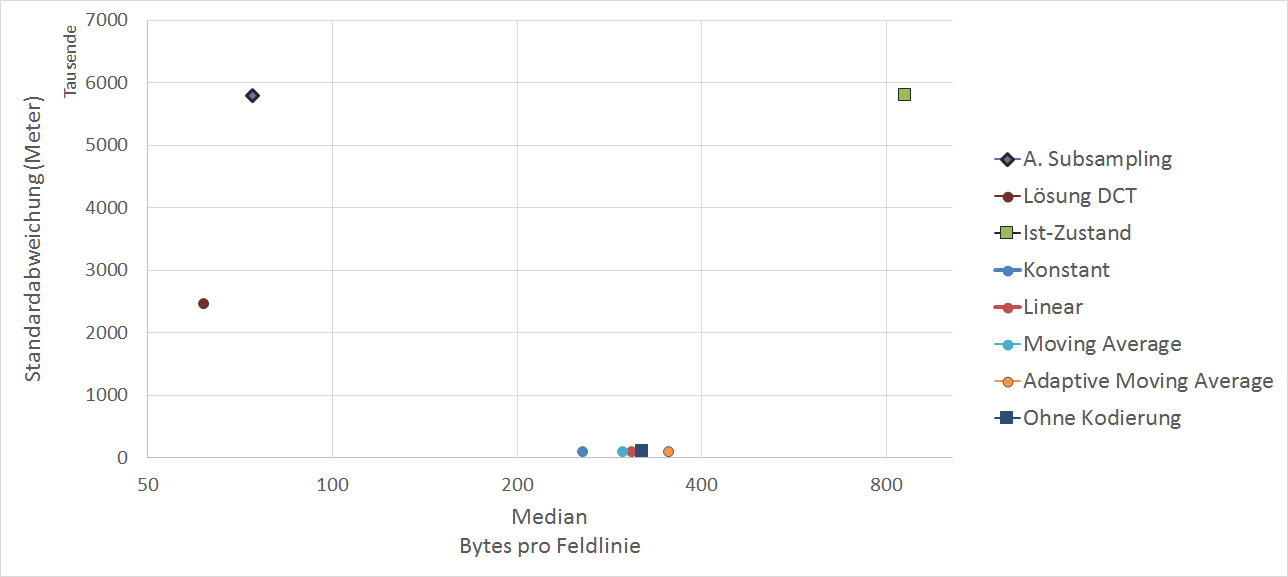
\includegraphics[width=1\textwidth,keepaspectratio]{./pictures/resultate/loesung2/variante0/resultate.png}
	\caption{Kompressionsraten der vier Prediktoren im Vergleich zum Ist-Zustand}
	\label{resultate:loesung2:simple:resultate}
\end{figure}
Im Diagramm der Abbildung \ref{resultate:loesung2:simple:resultate} sind die Kompressionsraten der jeweiligen Prediktoren dargestellt. Ein Diagramm mit der PSNR-HVS-M wurde nicht erstellt. Sie ist für alle Prediktoren gleich und liegt bei $140.7$ dB. Unerwartet ist, dass der Konstante Prediktor mit $255$ Bytes pro Feldlinie die beste Kompression erreichte, obwohl die Daten nicht zuverlässig vorhersagen kann. Im Vergleich mit dem Moving Average Prediktor sind die Fehler der Vorhersagen bis zu $5$ Mal grösser, verbrauchen aber $40$ Bytes weniger um eine Feldlinie abzuspeichern. Der Fehler bleibt jedoch Konstant. Eine Möglichkeit ist, dass die Rar Kodierung sich wiederholende Muster findet.\\
Eine mögliche Optimierung ist die Adaptive Byte Kodierung der DCT-Variante, beschrieben im Abschnitt \ref{konzept:loesung1:kodierung}. Das Diagramm der Abbildung \ref{resultate:loesung2:simple:resultate_byte} zeigt die Resultate mit der Byte Kodierung. Der Konstante Prediktor verbraucht mit der Adaptiven Kodierung mehr Speicherplatz. Die Kompressionsrate der anderen Prediktoren wird durch die Adaptive Kodierung deutlich verbessert. Der Lineare Prediktor erreicht mit $214$ Bytes pro Feldlinie die beste Kompression. Das bedeutet, dass die Fehler des Konstanten Prediktors grösser sind, als die der anderen Prediktoren. Es bestätigt die Vermutung, dass die anderen Prediktoren die Daten besser vorhersagen können. Die Kompressionsrate des Konstanten Prediktors ist auf die Rar Kodierung zurückzuführen, welche in den Prediktor-Fehler Muster erkennen und effizient kodieren kann.\\ 
\begin{figure}[!htbp]
	\center
	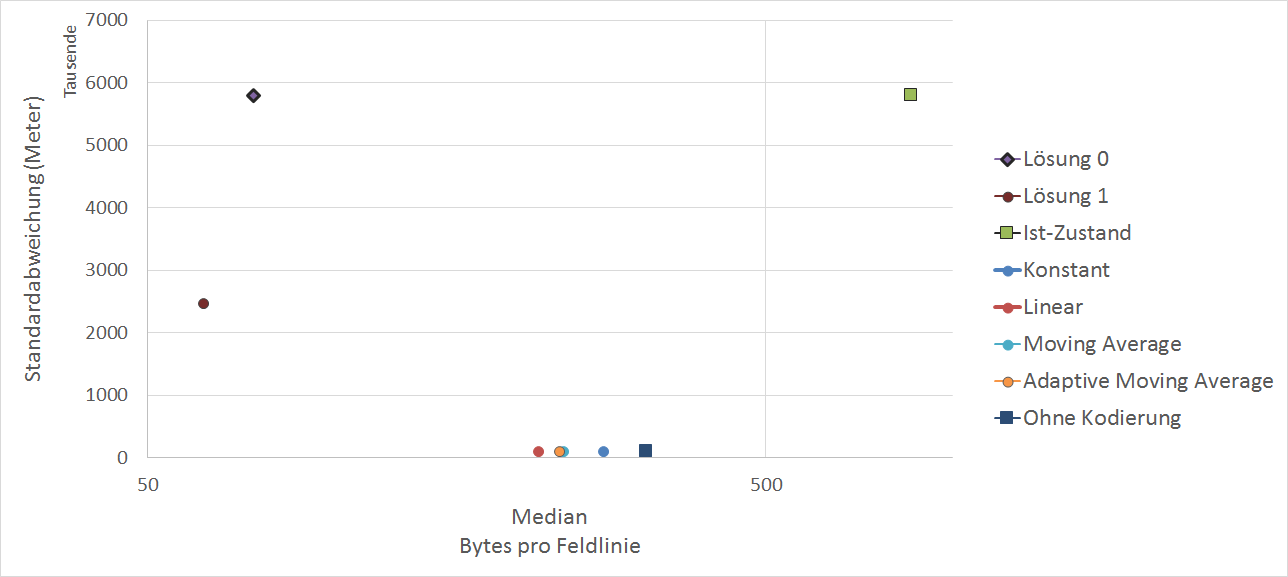
\includegraphics[width=1\textwidth,keepaspectratio]{./pictures/resultate/loesung2/variante0/resultate_byte.png}
	\caption{Artefakte der abschliessenden Variante. Links ohne Glättung, rechts mit Glättung}
	\label{resultate:loesung2:simple:resultate_byte}
\end{figure}
Der Linare Prediktor kann eine Feldinie mit etwa $214$ Bytes darstellen, was eine Kompressionsrate von $4$ ergibt. Auf kosten der Qualität wird versucht eine bessere kompressionsrate zu erreichen.

\subsubsection{Variante: Adaptiven Subsampling}
Gute Möglichkeit viele informationen zu verlieren.
Figure
schwieriger zu quantisieren, da weniger Stetig. Kurven der PCA. Möglichkeit eine Variante Prediktive kodierung für Kurven, wird aber einiges komplexer.
Einfacher wenn Kodierung für
Figure
Sphärisches Koordinatensystem.Einfacher abzuspeichern
POW
Aber Ebenfalls schwer vorherzusagen

\subsubsection{Wavelet Prediktive Kodierung}
beschrieben im Abschnitt \ref{konzept:prediktiv}
figure
figure psnr-hvs-m
